\documentclass[tikz, border=3pt]{standalone}

\usepackage{amsmath,amssymb}
\usepackage{pgfplots}
\pgfplotsset{compat=1.18}
\usepgfplotslibrary{groupplots}
\usetikzlibrary{arrows.meta}
\usepackage{xcolor}

\definecolor{utnblue}{RGB}{0, 51, 102}

\pgfplotsset{
    secuencia/.style={
        axis lines=middle,
        width=6.6cm, height=4.4cm,
        xmin=-1.6, xmax=6.6,
        ymin=-0.3, ymax=1.55,
        xtick={-1,1,2,3,4,5,6},
        ytick={0.5,1},
        yticklabels={$0{,}5$, $1$},
        tick label style={font=\tiny},
        label style={font=\scriptsize},
        title style={font=\scriptsize, at={(axis description cs:1,1)},
                     anchor=north east, xshift=-2pt, yshift=-2pt},
        xticklabel style={fill=white, inner sep=1.5pt},
        every axis x label/.style={at={(ticklabel* cs:1)}, anchor=west},
        every axis y label/.style={at={(ticklabel* cs:1)}, anchor=south},
        enlargelimits=false,
        clip mode=individual,
    },
}

\begin{document}
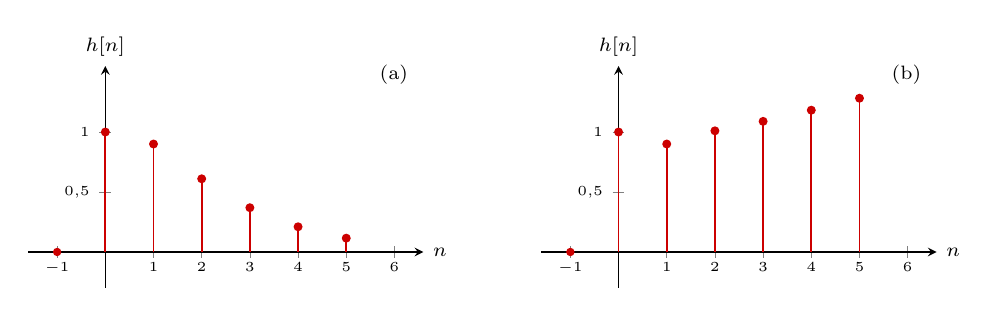
\begin{tikzpicture}[font=\scriptsize]

\begin{groupplot}[
    group style={group size=2 by 1, horizontal sep=1.5cm},
    secuencia,
]

% ---------------- (a) coeficiente -0,2 ----------------
\nextgroupplot[title={(a)}, ylabel={$h[n]$}, xlabel={$n$}]
\addplot[ycomb, red!80!black, semithick, mark=*, mark size=1.3pt,
         mark options={fill=red!80!black, draw=red!80!black}]
    coordinates {(0,1) (1,0.9) (2,0.61) (3,0.369) (4,0.2101) (5,0.11529)};
\addplot[only marks, red!80!black, mark=*, mark size=1.3pt]
    coordinates {(-1,0)};

% ---------------- (b) coeficiente +0,2 ----------------
\nextgroupplot[title={(b)}, ylabel={$h[n]$}, xlabel={$n$}]
\addplot[ycomb, red!80!black, semithick, mark=*, mark size=1.3pt,
         mark options={fill=red!80!black, draw=red!80!black}]
    coordinates {(0,1) (1,0.9) (2,1.01) (3,1.089) (4,1.1821) (5,1.28169)};
\addplot[only marks, red!80!black, mark=*, mark size=1.3pt]
    coordinates {(-1,0)};

\end{groupplot}

\end{tikzpicture}
\end{document}
